\documentclass[xcolor=dvipsnames]{beamer}

\usetheme{Boadilla}

\newcommand{\bi}{\begin{itemize}}
\newcommand{\ei}{\end{itemize}}
\newcommand{\be}{\begin{enumerate}}
\newcommand{\ee}{\end{enumerate}}
\newcommand{\I}{\item}
\newcommand{\f}{\frame}
\newcommand{\ft}{\frametitle}

\title{Status of the Offline Software}
\subtitle{GlueX Collaboration Meeting}
\author[M.\ Ito]{Mark M.\ Ito}
\date{January 29, 2010}
\institute[JLab]{Jefferson Lab}

\begin{document}

\f{\titlepage}

\f{
\bi
\I Alternate B-Field Studies: see David's talk
\I Position-Dependent Position Resolution: Yves calculated the effect, David has implemented it
\I Multi-particle/multi-photon events: largely done, documentation needed
\I 12 GeV Project Schedule, Offline Computing\cite{project}
  \bi
  \I a Gantt chart
  \I the list of tasks and their attributes including work required and cost
  \I ``steps'' for offline activities
  \I a cost comparison between the old plan and the new
  \I a manpower profile for both Lab staff and contributed labor
  \ei
\ei
}

\f{
$$
  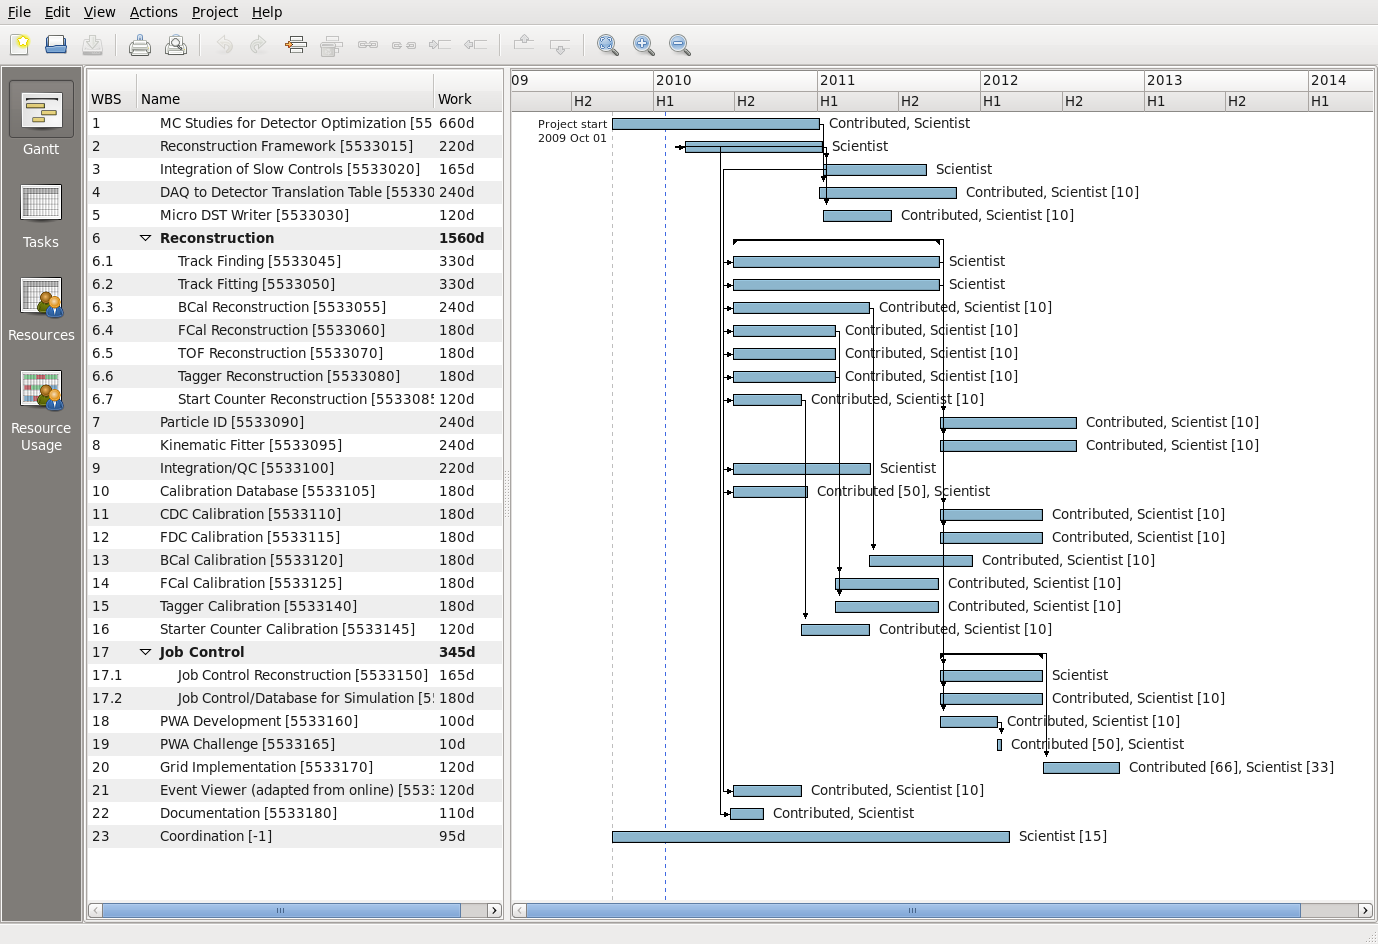
\includegraphics[height=3.2in]{HallDOfflineComputing.png}
$$
}


\f{
\bi
\I How Timing Is Done in GlueX: Craig Bookwalter working on this
  \bi
  \I prompted discussion on accessing the start counter geometry in reconstruction
  \I prompted changes in geometry interface: see David's talk
  \ei
\I New scheme for smearing FCAL hits: from David
  \bi
  \I now done in mcsmear rather than in the reconstruction
  \I BCAL smearing not migrated yet
  \ei
\I JLab batch farm priority:
  \bi
  \I negotiated an agreement with Hall B and the JLab Scientific computing
  \I Hall D gets increased priority on the JLab batch farm: 5\% $\rightarrow$ 20\%
  \I period of a week upon our request
  \ei
\I Coding Standards:
  \bi
  \I discussed and adopted
  \I enforcement regime not yet formalized
  \ei
\I Nightly builds are running: RHEL5, Fedora 8, CentOS 5\cite{nightly}
  \bi
  \I error reports mailed out once a week
  \ei
\I Geometry (HDDS) separated from src tree
  \bi
  \I Simplifies build scheme
  \I Exists as an extra package (a complication)
  \ei
\ei
}

\f{
\ft{Offline Task Priorities}
Priorities noted on task list\cite{tasks}
$$
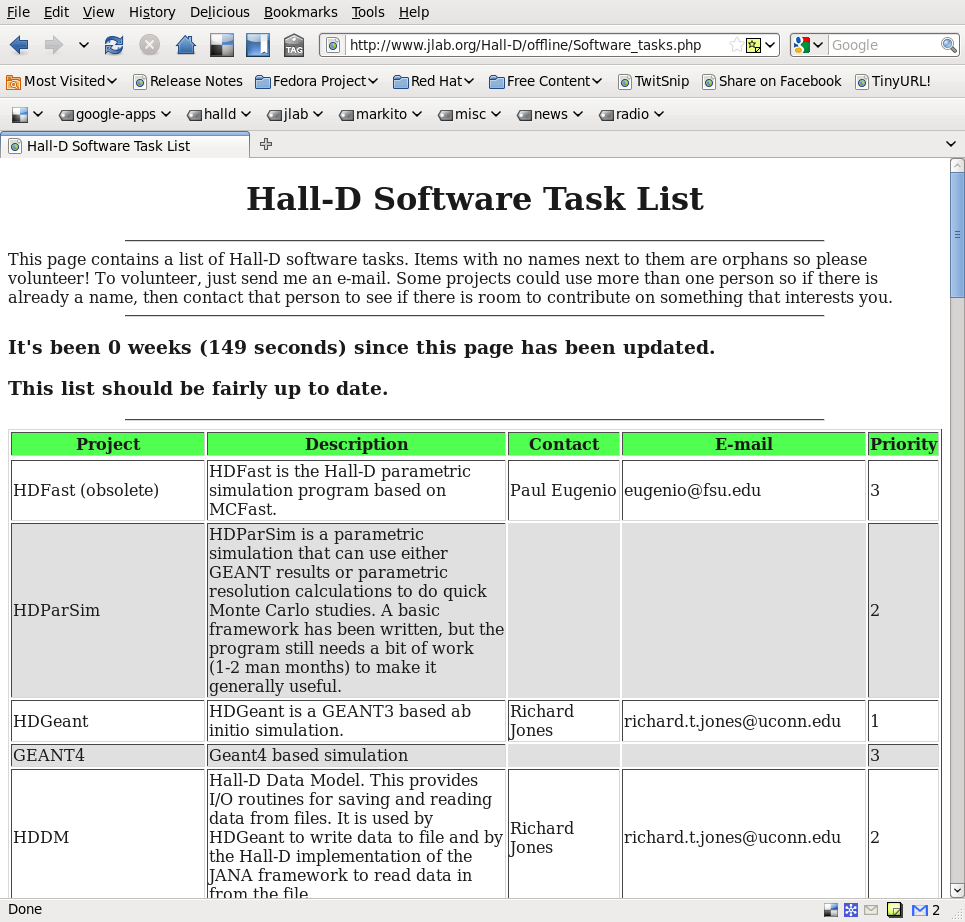
\includegraphics[height=3.0in]{SoftwareTaskList.png}
$$
}



\f{
\bi
\I Re-organization of high-level particle classes: see Simon's talk
\I Hall D Group Membership: old list cleaned up, Elliott
\I Parameterized B-field: David has started on this
\I Warning-Free Code Policy: adopted
\I New Subversion server
  \bi
  \I http service running on a new virtual machine
  \I running modern version of Subversion: v1.4
  \ei
\I Quick-start software builds: build automation\cite{quick-start}
\I Changes in dependency generation in the make scheme
\I Environment variable checking in the makefiles
\I New JANA version: many new features, see David's talk
\ei
}
\f{
\ft{References}
\begin{thebibliography}{99}
\tiny
\bibitem{tasks}http://www.jlab.org/Hall-D/offline/Software\_tasks.php
\bibitem{project}http://www.jlab.org/Hall-D/software/wiki/index.php/Offline\_Computing\_Project\_Management
\bibitem{nightly}http://www.jlab.org/Hall-D/software/wiki/index.php/Nightly\_Builds\_of\_GlueX\_Software
\bibitem{quick-start}http://www.jlab.org/Hall-D/software/wiki/index.php/Quick\_Start\_Guide\_to\_building\_GlueX\_Software
\end{thebibliography}
}

\end{document}

%%% end of latex file %%%%
